\documentclass[12pt]{article}
\usepackage{amsmath}
\usepackage[margin=2.5cm]{geometry}
\usepackage[utf8]{inputenc}
\usepackage{amsfonts}
\usepackage{fancyhdr}
\usepackage{hyperref}
\usepackage{graphicx}
\usepackage{caption}
\usepackage{subcaption}
\usepackage{setspace}
\usepackage{float}
\setstretch{1.3} 

%\usepackage{csc}% unknown package
\pagestyle{fancy}
\fancyhead[L]{Atmospheric Effects Modelling}
\fancyhead[R]{Page \thepage}
\fancypagestyle{firstpage}{%
  \lhead{}
  \rhead{}
}

\begin{document}
\begin{figure}[!tbp]
  \begin{subfigure}[b]{0.2 \textwidth}
    
\includegraphics[width=\textwidth]{img/uni}
  \end{subfigure}
  \hfill
  \begin{subfigure}[b]{0.25\textwidth}
    
\includegraphics[width=\textwidth]{img/fani}
  \end{subfigure}
\end{figure}
\begin{center}
\textbf{Atmospheric Effects Modelling} \\[1in]
Professor : Dr. Farzaneh\\~\\
St : AmirAbbas Saberi
\\[4in]
\textbf{University of Tehran}\\
November,27,2022
\end{center}
	\thispagestyle{firstpage}
\newpage
\textbf{Fermat's principle :}\\
Fermat's principle, also known as the principle of least time, is the link between ray optics and wave optics. In its original "strong" form, Fermat's principle states that the path taken by a ray between two given points is the path that can be traveled in the least time. In order to be true in all cases, this statement must be weakened by replacing the "least" time with a time that is "stationary" with respect to variations of the path — so that a deviation in the path causes, at most, a second-order change in the traversal time. To put it loosely, a ray path is surrounded by close paths that can be traversed in very close times. It can be shown that this technical definition corresponds to more intuitive notions of a ray, such as a line of sight or the path of a narrow beam.If points A and B are given, a wavefront expanding from A sweeps all possible ray paths radiating from A, whether they pass through B or not. If the wavefront reaches point B, it sweeps not only the ray path(s) from A to B, but also an infinitude of nearby paths with the same endpoints. Fermat's principle describes any ray that happens to reach point B; there is no implication that the ray "knew" the quickest path or "intended" to take that path. 
\begin{figure}[H]
	\centering
    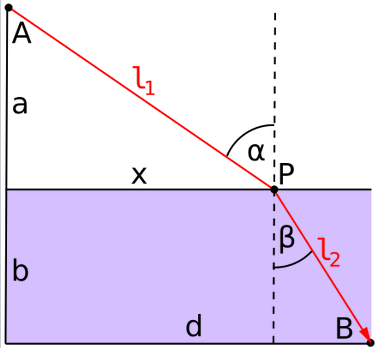
\includegraphics[width=0.2 \textwidth]{img/1}
    \caption{Beam refraction from A to B}
\end{figure}
since GPS signals are electromagnetic signals so they refract in layers of atmosphere.
 \begin{figure}[H]
	\centering
    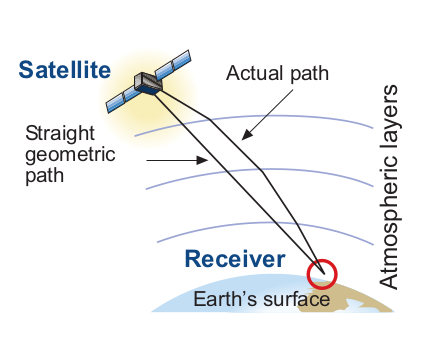
\includegraphics[width=0.4 \textwidth]{img/2}
    \caption{Path of signal in atmosphere layers}
\end{figure}
\newpage
Equation of distance is Euclidean, but ray path is not so it is one obligation to correct ray path to Euclidean line. \\
\centerline {$\Delta = \int_{ray path} n dl - \int_{straight line}dl = \int (n-1)dl$}\\
There are two parts in atmosphere , Ionosphere and Troposphere which their delays and effects are given as follows : \\ 
\section{Ionospheric Delay}
The ionosphere is that part of the terrestrial atmosphere that extends from
about 60 km up to more than 2000 km. As its name implies, it contains a
partially ionised medium, as a result of solar X- and Extreme UltraViolet
(EUV) rays in the solar radiation and the incidence of charged particles.
The propagation speed of GNSS electromagnetic signals in the iono-
sphere depends on its electron density (see below), which is typically driven
by two main processes. During the day, the Sun’s radiation ionises neutral
atoms to produce free electrons and ions. During the night, the recombi-
nation process prevails, where free electrons are recombined with ions to
produce neutral particles, which leads to a reduction in the electron density.\\
refractive index of the iono-
sphere can be approximated : \\
\centerline{$n_ph = 1-\frac{40.3}{f^2}N_e$}
\centerline{$n_gr = 1+\frac{40.3}{f^2}N_e$}
\centerline{$\Delta^{iono}_{ph,f} = -\frac{40.3}{f^2}\int N_e dl = -\alpha_f STEC$}
\centerline{$\Delta^{iono}_{gr,f} = +\frac{40.3}{f^2}\int N_e dl = \alpha_f STEC$}
\subsection{Ionospheric Models for Single-Frequency Receivers}
Single-frequency receivers need to apply a model to remove the ionospheric
refraction, which can reach up to few tens of metres, depending on the
elevation of rays and the ionospheric conditions.
\subsubsection{Klobuchar Model}
1- Calculate the Earth-centred angle \\
\centerline{$\psi = \pi/2 -E -arcsin(\frac{R_E}{R_E+h}cos(E))$}\\

2- Compute the latitude of the IPP \\
\centerline{$\phi_I = arcsin(sin(\phi_u)cos(\psi) + cos(\phi_u)sin(\psi)cos(A))$}\\
3- Compute the longitude of the IPP\\
\centerline{$\lambda_I = \lambda_u+\frac{\psi sin(A)}{cos(\phi_I)}$}
4- Find the geomagnetic latitude of the IPP\\
\centerline{$\phi_m = arcsin(sin(\phi_I)sin(\phi_P)+cos(phi_I)cos(phi_P)cos(\lambda_I-\lambda_P))$}

pole coordinate lat and long = 78.3 and 291.0 deg.\\
5- Find the local time at the IPP\\
\centerline{$t = 43200 \lambda_I/\pi + {t_{GPS}} $ and $\lambda_i$ radians and t in second} 
6- Compute the amplitude of ionospheric delay\\
\centerline{$A_I = \sum_{n = 0}^{3} \alpha_n(\phi_m/\pi)^n$  (seconds)}
if $A_I < 0 \rightarrow A_I = 0$.\\
7- Compute the period of ionospheric delay\\
\centerline{$P_I = \sum_{n=0}^3 \beta_n(\phi_m/\pi)$ (seconds)}
if $P_I < 72000 \rightarrow P_I = 72000$.\\
8- Compute the phase of ionospheric delay\\
\centerline{$X_I = \frac{2\pi(t-50400)}{P_I}$}
9- Compute the slant factor (ionospheric mapping function)\\
\centerline{$F = [1-(\frac{R_E}{R_E+h}cos(E))]$}
10- Compute the ionospheric time delay
\[
  I_1 = \begin{cases}
    [5.10^{-9} + A_Icos(X_I)]F & \text{if $|X_I| < \pi/2$} \\
    5.10^{-9}F & \text{if $|X_I| >= \pi/2$} \\
  \end{cases}
\]
Result : 
\begin{figure}[H]
	\centering
    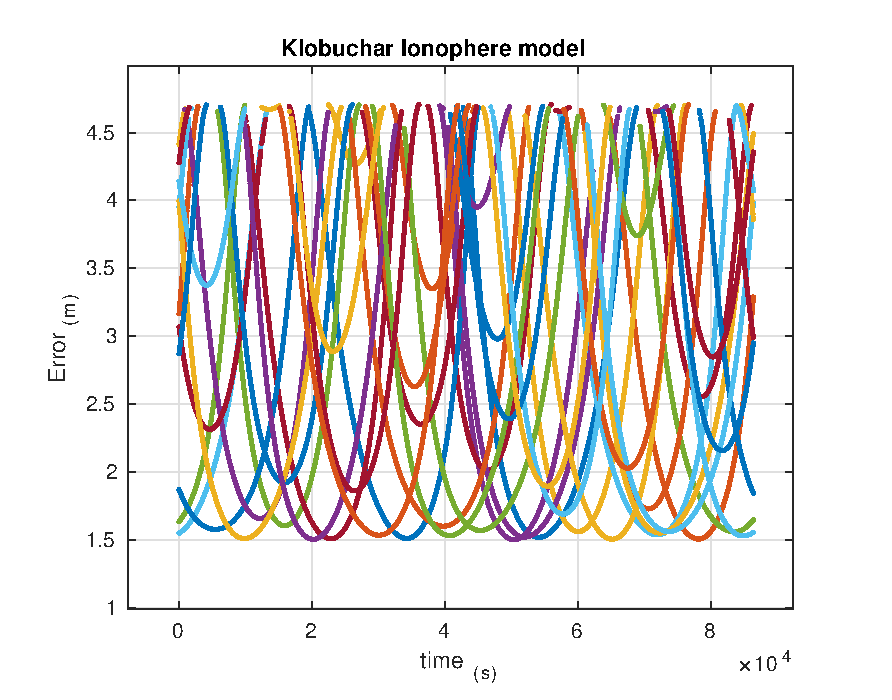
\includegraphics[width=0.43 \textwidth]{img/klo}
    \caption{Klobuchar model IZU satation in 2015}
\end{figure}
\newpage
\section{Tropospheric Delay}
The troposphere is the atmospheric layer between Earth’s surface and an
altitude of about 60 km.
The effect of the troposphere on the GNSS signals appears as an extra
delay in the measurement of the signal travelling from the satellite to the
receiver. This delay depends on the temperature, pressure and humidity
as well as the transmitter and receiver antenna locations.\\
\centerline{$Tr = \int (n-1)dl = \int N_{hydr} + N_{wet}$}
Hydrostatic component delay: This is caused by the dry gases present
in the troposphere (78% N2 , 21% O2 , 0.9% Ar, etc.). Its effect
varies with local temperature and atmospheric pressure in a quite
predictable manner, although its variation is less than 1% over a few
hours. The error caused by this component is about 2.3 m in the
zenith direction and 10 m for lower elevations\\
Wet component delay: This is caused by the water vapour and con-
densed water in the form of clouds and, therefore, it depends on the
weather conditions. The excess delay is small in this case, only some
tens of centimetres, but this component varies faster than the hydro-
static component and in a quite random way, thus being very difficult
to model.
\subsection{Collins Model}
there is a common mapping function for the wet and dry
troposphere : \\
\centerline{$Tr(E) = (Tr_{z,d}+Tr_{z,w})M(E)$}
\centerline{$M(E) = \frac{1.001}{\sqrt{0.002001+sin^2(E)}}$}
\centerline{$\zeta(\phi,D) = \zeta_0(\phi) - \Delta\zeta(\phi)cos[\frac{2\pi(D-D_{min}}{365.25}]$}
\centerline{$Tr_{z_0,d} = \frac{10^-6 k_1 R_d P}{g_m}$ , $Tr_{z_0,w} = \frac{10^- k2 Rd e}{(\lambda+1)g_m -\beta R_d T}$}
\centerline{$Tr_{z,d} = [1-\frac{\beta H}{T}]^{g/(R_d \beta)}Tr_{z_0,d}$}
\centerline{$Tr_{z,w} = [1-\frac{\beta H}{T}]^{(\lambda+1)g/(R_d \beta) -1}Tr_{z_0,w}$}
$k1 = 77.604 K/mbar$ , $k2 = 382000 K^2/mbar
$ , $Rd = 287.054 J/(kg K)$ , $g_m = 9.784 m/s^2 $, $g = 9.8 m/s^2$\\
\subsection{Hopfield}
\centerline{$ZHD = (0.62291/T+0.0023081)P$}
\centerline{$ZWD = (555.7+1.792 10^-4 exp((T-273)/22.9)) e/T^2$}
\centerline{$Tr_h =  (ZHD+ZWD)M$}
\subsection{Sustamiinen}
\centerline{$g = 1 - 0.0026 cosd(2\phi)-0.00000028 h_0$}
\centerline{$ pr = 1013.25;
 Tr = 18+273$}
\centerline{$ hr = 0;
 Hr = 50/100$}
\centerline{$ p = pr(1-0.0000226(h_0-hr))^5.225$}
\centerline{$ T = Tr - 0.0065(h_0-hr)$}
\centerline{$ H = H_r e.^(-0.0006396 (h_0-hr))$}
\centerline{$Tr_{dw} = \frac{0.002277}{g}(P+(1255./T+0.05)e)$}
\centerline{$Tr_s = (Tr_{dw})M$}

Result : 

\begin{figure}[H]
  \begin{subfigure}[b]{0.5 \textwidth}
    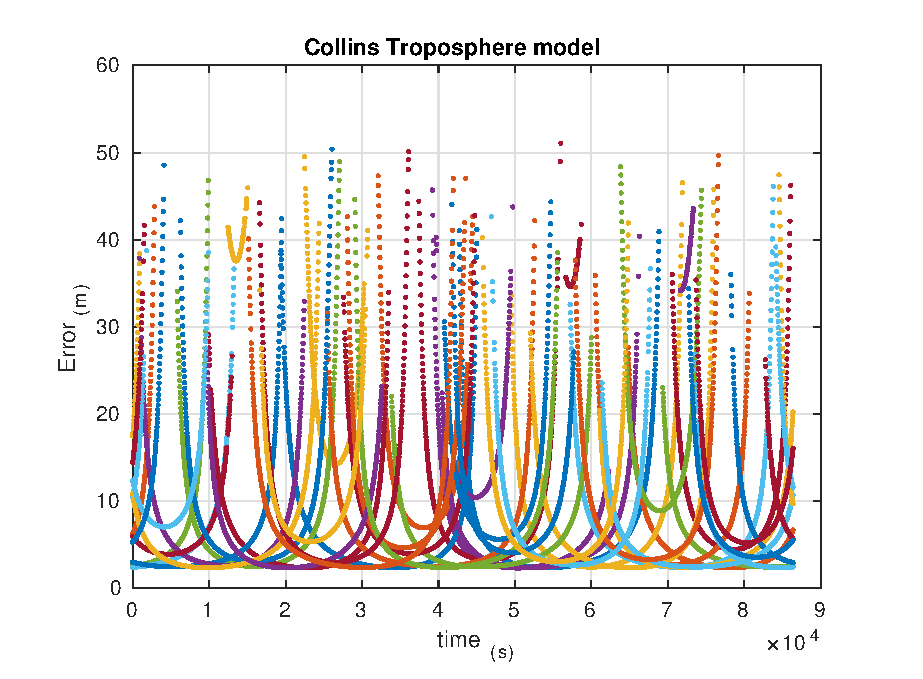
\includegraphics[width=\textwidth]{img/col}
  \end{subfigure}
  \hfill
  \begin{subfigure}[b]{0.5\textwidth}
    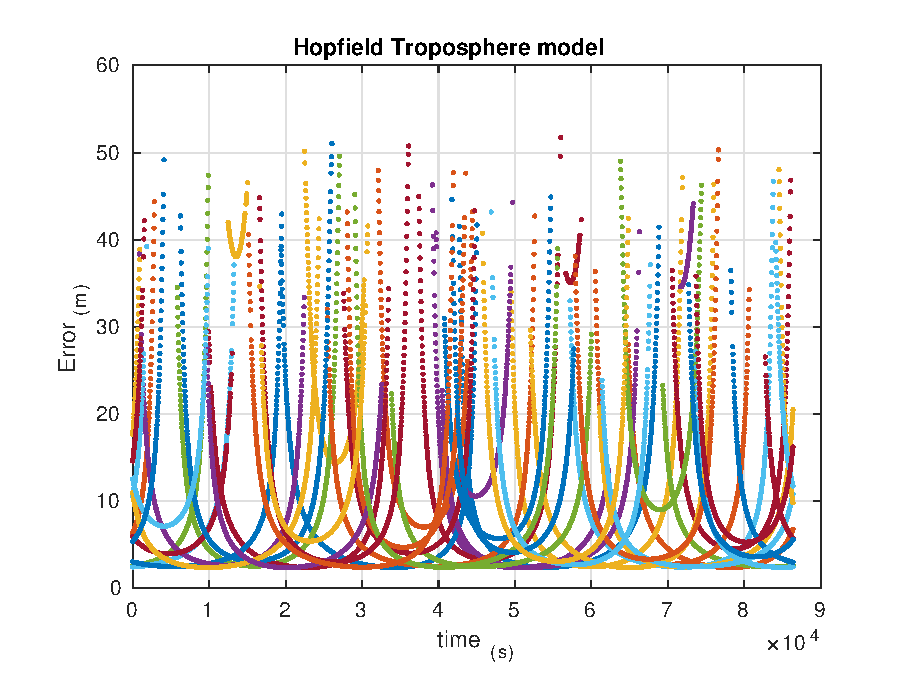
\includegraphics[width=\textwidth]{img/hop}
  \end{subfigure}
  \caption{Collins anf Hopfield model MIZU satation in 2015}
\end{figure}
\begin{figure}[H]
	\centering
    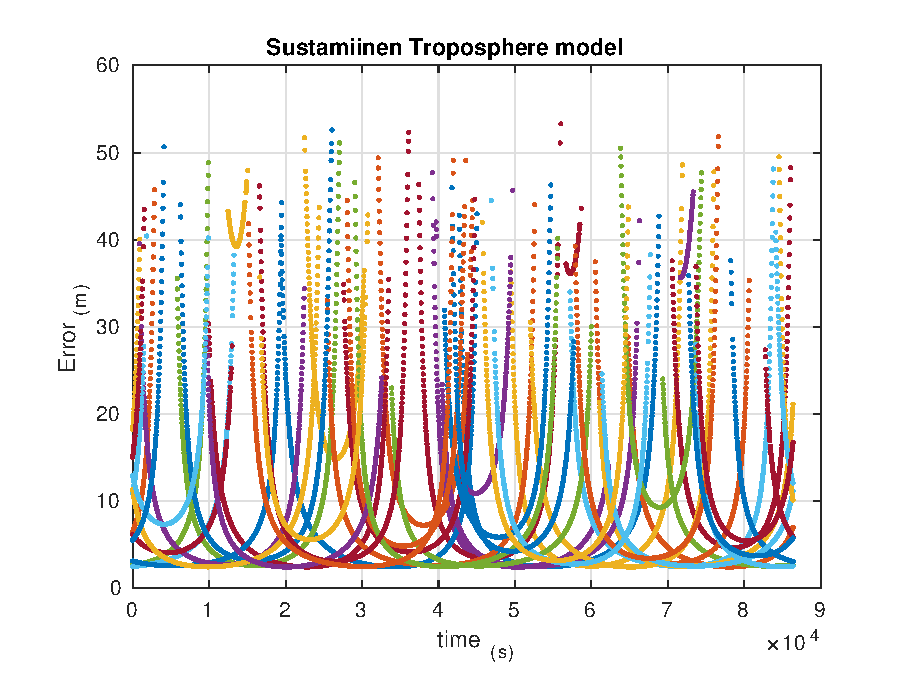
\includegraphics[width=0.5 \textwidth]{img/sus}
    \caption{Sustamiinen model MIZU satation in 2015}
\end{figure}
\end{document}










